\section{State-of-the-Art Review of XRL Methods}
\label{sec:state_of_the_art}
\begin{table*}[t]
% \footnotesize
\hspace*{\fill}
\resizebox{\textwidth}{!}{
\begin{tblr}{|Q[c,m]|Q[c,m,4cm]|Q[c,m,7cm]|Q[c,m]|Q[c,m]|Q[c,m]|}
    \hline
    \SetCell[r=2]{c} \hyperref[subsec:subject]{\textbf{Explanation \\ Target}} & \SetCell[r=2]{c} \hyperref[subsec:form]{\textbf{Explanation \\ Form}} & \SetCell[r=2]{c} \hyperref[sec:state_of_the_art]{\textbf{Explainability \\ Method}} & \SetCell[c=3]{} \hyperref[subsec:source]{\textbf{Source of \\ Explanation}} & & \\
    \hline
    & & & \rotatebox{-90}{\shortstack{Policy}} & \rotatebox{-90}{\shortstack{Trajectories}} & \rotatebox{-90}{\shortstack{Value \\ functions}} \\
    \hline
    \hline
    \SetCell[r=6]{c} Decision & \SetCell[r=2]{c} \hyperref[subsec:policy_model]{{Policy Model}} & \hyperref[subsubsec:interpretable_policy_learning]{{\textit{Interpretable policy learning}}} & \scalebox{2}{\checkmark} & & \\
    \hline
    & & \hyperref[subsubsec:policy_approximation_via_interpretable_model]{{\textit{Policy approximation via interpretable model}}} & \scalebox{2}{\checkmark} & & \\
    \hline
    & \SetCell[r=3]{c} \hyperref[subsec:saliency_map]{{Saliency Map}} & \hyperref[subsubsec:observation_perturbation]{\textit{Observation perturbation}} & \scalebox{2}{\checkmark} & & \\
    \hline
    & & \hyperref[subsubsec:observation_gradient_analysis]{\textit{Observation gradient analysis}} & \scalebox{2}{\checkmark} & & \\
    \hline
    & & \hyperref[subsubsec:attention_based_architecture]{\textit{Attention-based architecture}} & \scalebox{2}{\checkmark} & & \\
    \hline
    & \hyperref[subsec:counterfactual]{{Counterfactual}} & \hyperref[subsubsec:latent_space_counterfactual_generation]{\textit{Latent space usage for counterfactual generation}} & \scalebox{2}{\checkmark} & & \\
    \hline
    \hline
    \SetCell[r=7]{c} Strategy & \SetCell[r=2]{c} \hyperref[subsec:trajectory_prediction]{{Trajectory Prediction}} & \hyperref[subsubsec:value_functions_as_observations]{{\textit{Value functions as observations}}} & & & \scalebox{2}{\checkmark} \\
    \hline
    & & \hyperref[subsubsec:critic_enrichment]{\textit{Critic enrichment}} & & & \scalebox{2}{\checkmark} \\
    \hline
    & \SetCell[r=2]{c} \hyperref[subsec:interaction_model]{{Interaction Model}} & \hyperref[subsubsec:bayesian_network_learning]{\textit{Bayesian network learning}} & & \scalebox{2}{\checkmark} & \\
    \hline
    & & \hyperref[subsubsec:latent_space_mdp_generation]{{\textit{Latent space usage for MDP generation}}} & \scalebox{2}{\checkmark} & & \\
    \hline
    & \SetCell[r=3]{c} \hyperref[subsec:agent_trajectory]{{Agent Trajectory}} & \hyperref[subsubsec:hierarchical_decomposition]{\textit{Hierarchical decomposition}} & \scalebox{2}{\checkmark} & & \\
    \hline
    & & \hyperref[subsubsec:extraction_via_critic_analysis]{\textit{Extraction via critic analysis}} & & \scalebox{2}{\checkmark} & \scalebox{2}{\checkmark} \\
    \hline
    & & \hyperref[subsubsec:extraction_via_multi_critic_comparisons]{\textit{Extraction via multi-critic comparisons}} & & \scalebox{2}{\checkmark} & \scalebox{2}{\checkmark} \\
    \hline
\end{tblr}
}
\hspace*{\fill}
\caption{Taxonomy of explainability methods in reinforcement learning.}
\label{tab:taxonomy_methods}
\end{table*}


The purpose of this section is to detail the functioning of existing explainability methods (see Table~\ref{tab:taxonomy_methods}).
They are presented according to the form of explanation they produce, following the taxonomy introduced in Section~\ref{sec:taxonomy_xrl_methods}.

Each subsection introduces one of the six forms of explanation identified in Section~\ref{subsec:form}.
For each form, we identify the corresponding family of methods and organize the related approaches within the appropriate subsection.
A family of methods is defined as a set of methods that share the same source, form, and subject of explanation, as well as a similar procedure for generating explanations.
Methods belonging to the same family may differ slightly in their implementation or in the details of the generation process.
They share a common underlying principle that allows them to be described as part of the same family.

\subsection{Policy Model}
\label{subsec:policy_model}

The policy function can be represented by a wide variety of function classes.
In modern reinforcement learning, neural networks is the most commonly used models for representing policies.
Although these models achieve the highest performance, their connectionist nature makes their internal representations non-interpretable.

For this reason, a substitutive approach to XRL aims to replace these models with alternative models considered interpretable.
Such models can be understood through direct analysis of their representations.
The main classes of interpretable models used to represent policy functions include decision trees \cite{topin2021iterative}, algorithms \cite{trivedi2022learning}, formal logic \cite{payani2019inductive}, and linear models \cite{pmlr-v108-garreau20a}.

Explanations derived from an interpretable model primarily provide insights into the decision-making process, since what is modeled is the mapping between an observation and an action.
If the model is sufficiently simple or well structured, the observer can form a mental representation of a sequence of decisions across the environment and thus obtain information about the agent's strategy.

The main limitation of these methods is that interpretable models rely on symbolic representations.
When the policy to be represented is too complex, achieving comparable performance requires a large number of rules or conditions.
The resulting model can quickly become difficult to analyze and lose its interpretability.


For example, representing a policy capable of playing Go using a symbolic model would require considering a very large number of possible situations and specific cases.
Even if such a representation were possible, the resulting model would likely become intractable for human analysis due to its complexity.
This illustrates why neural network-based approaches have become dominant in such domains, as they can learn complex decision strategies without requiring an explicit enumeration of rules.

To obtain an interpretable policy model, two explainability methods are available: \textit{interpretable policy learning} and \textit{policy approximation via interpretable model}.

\subsubsection{\textit{Interpretable Policy Learning}}
\label{subsubsec:interpretable_policy_learning}

This method aims at learning a policy represented by an \textbf{interpretable} model \cite{topin2021iterative, trivedi2022learning}.
It is the most direct approach to addressing the challenges posed by explainable reinforcement learning (XRL).
This type of training requires modifying the MDP in order to adapt it to the search space and to the type of policy representation.
Moreover, this search space often needs to be reduced to make learning feasible.
Such a \textbf{reduction} requires the integration of \textbf{expert knowledge} into the learning process.
With this method, the \textit{interpretable policy function} itself is used to provide explanations to the observer.

\subsubsection{\textit{Policy Approximation via Interpretable Model}}
\label{subsubsec:policy_approximation_via_interpretable_model}

Using an interpretable model, it is possible to \textbf{approximate} a non-interpretable policy \cite{sieusahai2021explaining}.
In this setting, the problem is cast as a \textbf{supervised learning} task, where the non-interpretable policy is used to label each observation with the action it selects.
Using this dataset, supervised learning is then performed with the interpretable model.
The resulting \textit{interpretable model} is subsequently used as an explanation for the observer.
If this approximation is sufficiently faithful, it can be deployed in the environment in place of the original policy, thereby enabling a high degree of control over the agent.

\subsection{Saliency Map}
\label{subsec:saliency_map}

\begin{figure}[t]
    \centering
    \begin{subfigure}[b]{0.4\textwidth}
        \centering
        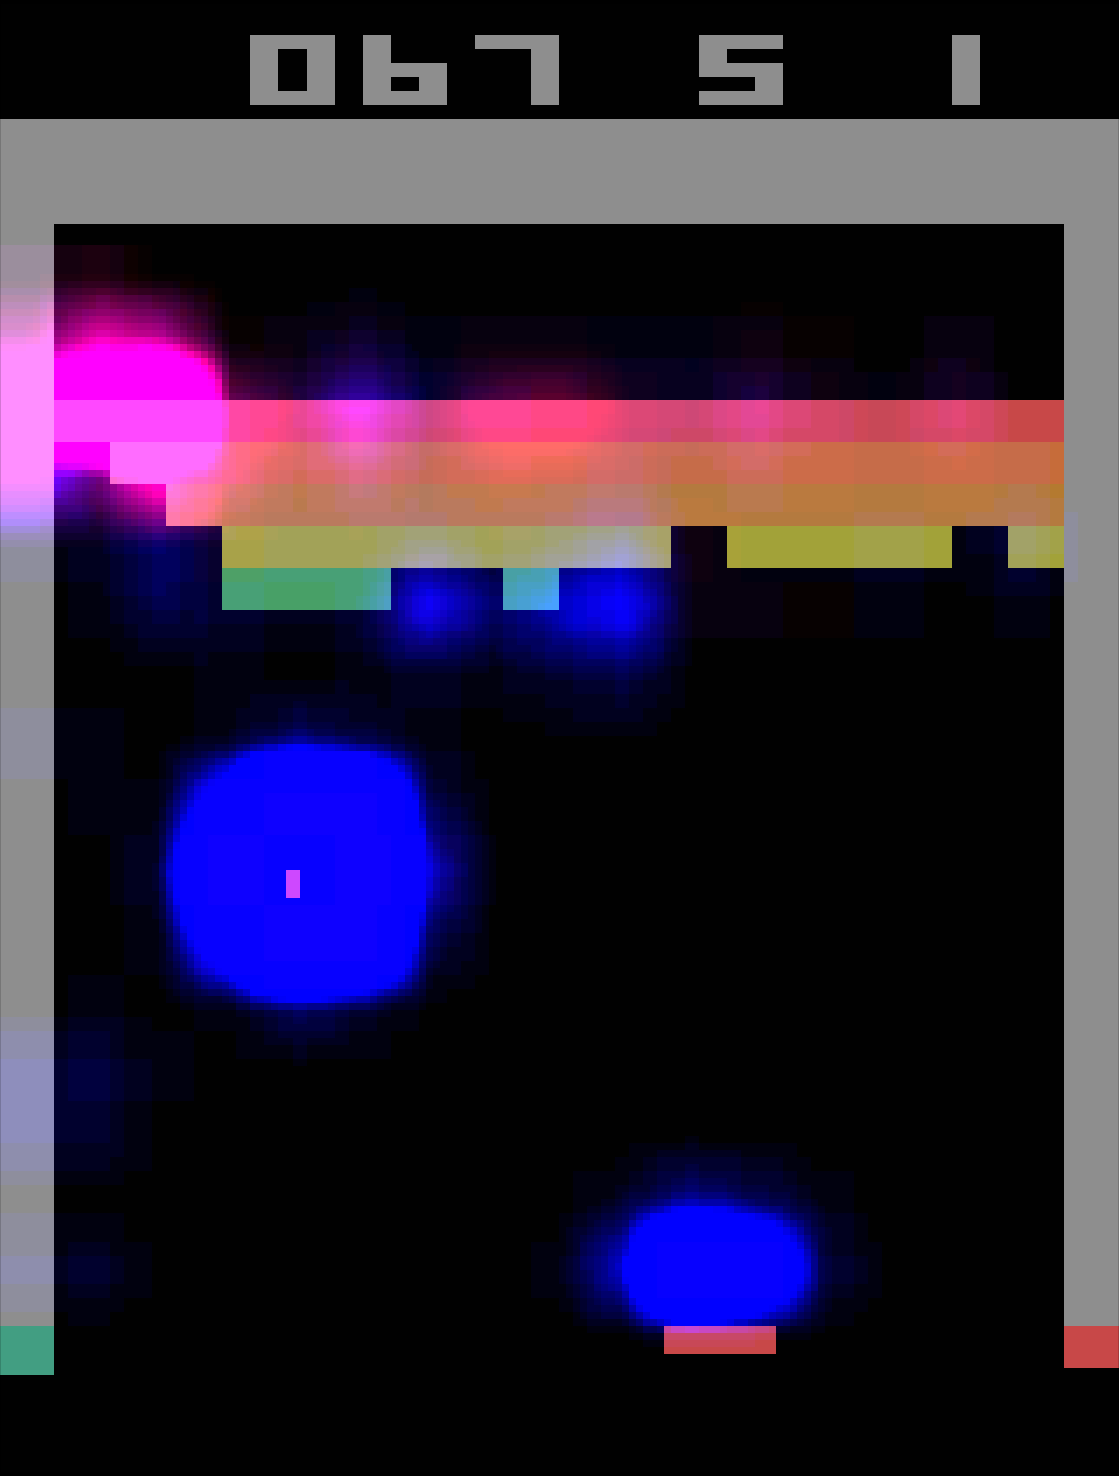
\includegraphics[width=\textwidth]
            {figures/explainability_reinforcement_learning/hit_map_1.png}
        \caption{}
        \label{fig:saliency_map_heatmap_perturbation}
    \end{subfigure}
    \hspace{0.02\textwidth}
    \begin{subfigure}[b]{0.4\textwidth}
        \centering
        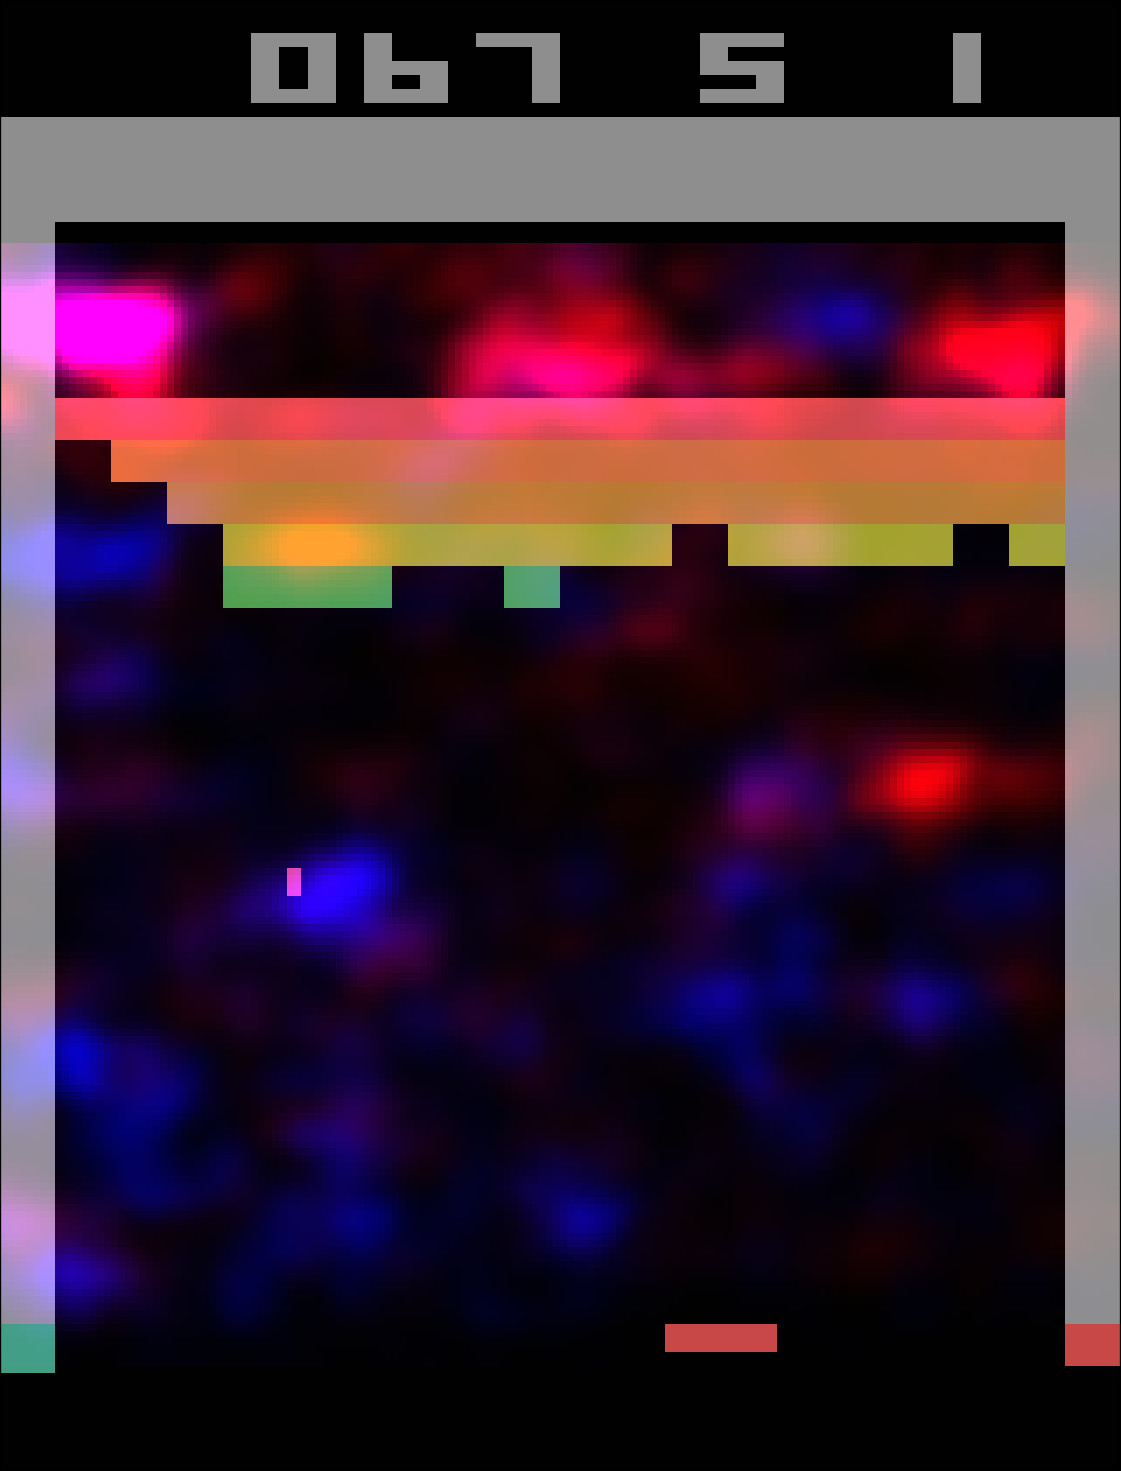
\includegraphics[width=\textwidth]
            {figures/explainability_reinforcement_learning/hit_map_2.png}
        \caption{}
        \label{fig:saliency_map_heatmap_gradient}
    \end{subfigure}
    \caption{
        Heatmaps for the same observation of the Atari game ``Breakout'' \cite{greydanus2018visualizing}.
    }
    \label{fig:saliency_map_heatmap}
\end{figure}


Heatmaps make it possible to identify which parts of the input vector are decisive in the selection of the output (as illustrated in Figure~\ref{fig:saliency_map_heatmap}).
When applied to the reinforcement learning setting, they highlight the regions of the observation space that are critical in the action selection process.
By nature, this form of explanation provides information about the policy's decision-making process.
The intuitive nature of this representation allows it to be used by a broad audience.

A limitation of heatmap-based methods is that the resulting explanations are not always directly meaningful to the observer.
As illustrated in Figure~\ref{fig:saliency_map_heatmap_gradient}, interpreting which regions are important often requires human reasoning and involves a degree of subjectivity.
This limitation becomes particularly relevant in reinforcement learning, where the objective is not only to explain a single decision but also to understand the factors influencing a sequence of decisions over time.

More generally, heatmap-based methods highlight a fundamental challenge in XAI: determining the relevance of an explanation.
Different methods can produce different heatmaps for the same decision, raising the question of how to compare and select among potentially conflicting explanations.
This is illustrated in Figure~\ref{fig:saliency_map_heatmap}, where the perturbation-based method (Figure~\ref{fig:saliency_map_heatmap_perturbation}) and the gradient-based method (Figure~\ref{fig:saliency_map_heatmap_gradient}) produce different heatmaps for the same observation.
Rather than assuming that only one explanation can be valid, the definition of explanation adopted in this manuscript allows for multiple complementary perspectives.
Different explanations may reveal different aspects of the system and contribute to improving the observer's understanding.

Three explainability methods can be used to obtain this type of explanation: \textit{observation perturbation}, \textit{observation gradient analysis}, and \textit{attention-based architectures}.

\subsubsection{\textit{Observation Perturbation}}
\label{subsubsec:observation_perturbation}

Perturbation analysis consists in applying various \textbf{modifications} to the observation in order to study their \textbf{impact} on the output of the \textbf{policy function} \cite{greydanus2018visualizing}.
The greater the variation in the output caused by a perturbation applied to a given component of the input vector, the higher the \textbf{weight} assigned to that component.
The magnitude of the perturbation is measured by computing the distance between the original output and the output obtained from the perturbed input.
Using this set of weights, a \textit{heatmap} is constructed, enabling the observer to visualize which parts of the observation vector are most sensitive in the action-selection process (see Figure~\ref{fig:saliency_map_heatmap_perturbation}).

\subsubsection{\textit{Observation Gradient Analysis}}
\label{subsubsec:observation_gradient_analysis}

Observation \textbf{gradient} analysis refers to a set of methods that require a differentiable policy function in order to extract information from it \cite{simonyan2014deep, weitkamp2019visual, huber2019enhancing}.
To this end, the gradient of the policy function is computed with respect to all \textbf{components of the input vector}.
For each input component, the resulting gradient provides a weighting that represents its importance in the output of the policy function.
Based on these weightings, a \textit{heatmap} is constructed to allow the observer to visually identify the parts of the input vector that are the most influential in the policy function's output (see Figure~\ref{fig:saliency_map_heatmap_gradient}).

\subsubsection{\textit{Attention-Based Architecture}}
\label{subsubsec:attention_based_architecture}

\begin{figure}[t]
    \centering
    \begin{subfigure}[b]{0.4\textwidth}
        \centering
        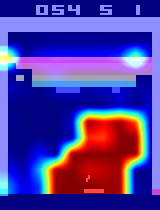
\includegraphics[width=\textwidth]
            {figures/explainability_reinforcement_learning/attention_map_1.png}
        \caption{}
        \label{fig:attention_map_heatmap_clear}
    \end{subfigure}
    \hspace{0.02\textwidth}
    \begin{subfigure}[b]{0.4\textwidth}
        \centering
        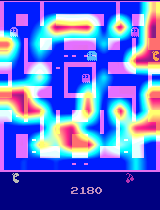
\includegraphics[width=\textwidth]
            {figures/explainability_reinforcement_learning/attention_map_2.png}
        \caption{}
        \label{fig:attention_map_heatmap_unclear}
    \end{subfigure}
    \caption{
        Attention-based heatmaps for the Atari games ``Breakout'' and ``Ms.\ Pac-Man'' \cite{mott2019towards}.
    }
    \label{fig:attention_map_heatmap}
\end{figure}


\textbf{Attention} blocks constitute a neural network architecture that makes it possible to weight the relative importance of one part of a vector with respect to the other parts of the same vector \cite{vaswani2023attention}.
These weights are computed as a function of the vector itself and are learned by the neural network during training.
For a given observation, each component of the observation vector is assigned a scalar value.
It can therefore be assumed that the components associated with the highest weights are the most influential in determining the output \cite{mott2019towards, itaya2021visual}.
This attention-based \textit{heatmap} is then provided to the observer as the explanation (see Figure~\ref{fig:attention_map_heatmap_clear}).
However, as shown in Figure~\ref{fig:attention_map_heatmap_unclear}, the attention weights are not always concentrated on a small, easily interpretable set of regions, which can make this type of explanation difficult to exploit.

\subsection{Counterfactual}
\label{subsec:counterfactual}

\begin{figure}[t]
    \centering
    \begin{subfigure}[b]{0.35\textwidth}
        \centering
        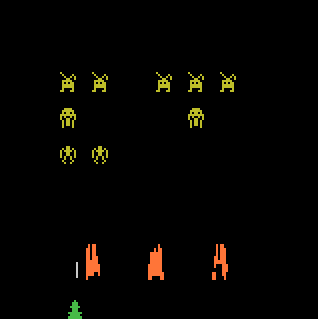
\includegraphics[width=\textwidth]
            {figures/explainability_reinforcement_learning/contrefactuel_1.png}
        \caption{}
        \label{fig:counterfactual_example_original}
    \end{subfigure}
    \hspace{0.02\textwidth}
    \begin{subfigure}[b]{0.35\textwidth}
        \centering
        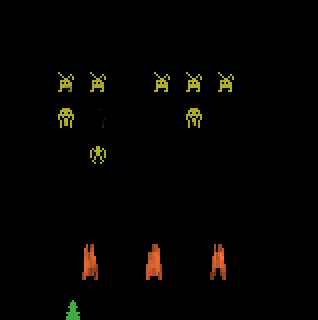
\includegraphics[width=\textwidth]
            {figures/explainability_reinforcement_learning/contrefactuel_2.png}
        \caption{}
        \label{fig:counterfactual_example_counterfactual}
    \end{subfigure}
    \caption{
        Counterfactual explanation of the agent's behavior for the Atari game \textit{Space Invaders} \cite{olson2021counterfactual}.
        Panel~\subref{fig:counterfactual_example_original} shows the original observation and panel~\subref{fig:counterfactual_example_counterfactual} the counterfactual observation produced by a generative model.
    }
    \label{fig:counterfactual_example}
\end{figure}


In the context of reinforcement learning, counterfactual explanations are used to generate new observations (see Figure~\ref{fig:counterfactual_example}).
This new observation, distinct from the original one, leads the agent to adopt an alternative behavior.
A counterfactual explanation aims to explain the agent's decision-making process.
Modifying the observation informs the observer about the adjustments required for the agent to adopt a different behavior.
The method available to generate counterfactuals is the \textit{use of the latent space for counterfactual generation}.

\subsubsection{\textit{Latent Space Usage for Counterfactual Generation}}
\label{subsubsec:latent_space_counterfactual_generation}

In this method, \textbf{generative models} are used \cite{bond2021deep} to exploit the latent representation.
This type of model learns to generate new data by imitating the training data distribution.
In this context, generative models aim to produce alternative observations that are likely to alter the agent's actions \cite{olson2021counterfactual}.

The main challenge of this approach lies in the fact that, to serve as explanations, counterfactuals must be both \textbf{close} and \textbf{feasible}.
A close counterfactual refers to one that does not differ significantly from the original observation.
A feasible counterfactual corresponds to an observation that is meaningful within the considered environment.

\subsection{Agent Trajectory}
\label{subsec:agent_trajectory}

Trajectories represent a sequence of interactions between the agent and its environment.
By analyzing these trajectories, the observer can infer the underlying dynamics governing the agent's evolution within its environment.

Post-training trajectories are systematically used to obtain explanations of the agent's strategy, even outside the scope of explainable reinforcement learning (XRL).
This simple approach can be enhanced using methods such as \textit{hierarchical decomposition} and \textit{extraction via critic analysis}.

Training trajectories, on the other hand, can be used to explain the agent's learning process, through the \textit{extraction via multi-critic comparisons} method.

\subsubsection{\textit{Hierarchical Decomposition}}
\label{subsubsec:hierarchical_decomposition}

Hierarchical agents are composed of a set of \textbf{sub-policies} specialized for specific tasks within subsets of the environment's states.
This method distributes the optimization of the reward function across multiple models, significantly simplifying the learning process.
Moreover, this \textbf{decomposition} of the policy function can also provide explainability in the agent's strategy \cite{Beyret_2019}.
If a sub-policy is selected, it indicates that the agent will execute a specialized behavior.
This behavioral specialization provides insight into the strategy the agent employs to maximize the reward function.
The agent's \textit{trajectory}, together with the \textit{sub-policy} selected for each action, is used as interpretable information.

\subsubsection{\textit{Extraction via Critic Analysis}}
\label{subsubsec:extraction_via_critic_analysis}

In this method, the predictions of the critic are used to determine which \textbf{trajectories to present to the observer} \cite{Sequeira_2020}.
A set of states is selected from multiple trajectories.
For a given state, all possible actions are examined.
The state is assigned a value equal to the difference between the critic's prediction for the lowest-valued action and the prediction for the highest-valued action.
Trajectories containing the states with the highest values according to this procedure are then chosen to be presented to the observer.
These trajectories are considered \textbf{critical moments} of the agent and are therefore relevant for analysis.
For this method, the \textit{selected trajectories} represent the interpretable information provided to the observer.

\subsubsection{\textit{Extraction via Multi-Critic Comparisons}}
\label{subsubsec:extraction_via_multi_critic_comparisons}

In this approach, the main objective is to \textbf{weight the training interactions} between the agent and the environment according to their influence on the learning process.
To achieve this, multiple critic functions are created using \textit{off-policy} learning.
Off-policy learning is a reinforcement learning process that allows a policy to learn from data generated by a different policy \cite{gottesman2020interpretable}.
Each critic function is trained on a subset of the dataset.

A reference critic function is trained using the entire dataset.
Then, for each agent-environment interaction, a critic function is retrained while specifically excluding that interaction.
The \textbf{prediction disparity} between the retrained critic and the reference critic represents the impact of removing that interaction on learning.
Through this procedure, a value is assigned to each interaction based on this difference: the larger the disparity, the higher the value assigned to the interaction.

A higher value indicates that the interaction is considered more important in the learning process.
These \textit{values} over the \textit{interactions} serve as explanations for the observer, providing a means to assess the significance of each agent-environment interaction within the learning process.

\subsection{Trajectory Prediction}
\label{subsec:trajectory_prediction}

\begin{figure}[t]
    \centering
    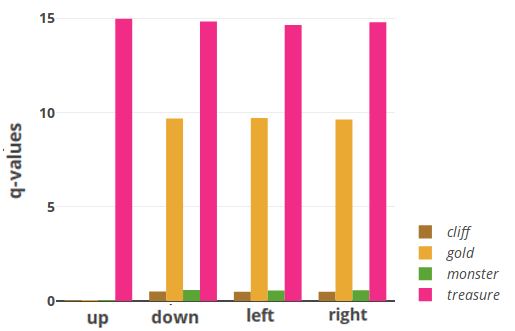
\includegraphics[width=0.6\textwidth]
        {figures/explainability_reinforcement_learning/multi_q_values.png}
    \caption{
        Prediction of sub-rewards as a function of the action selected by the
        agent for a given state \cite{juozapaitis2019explainable}. Depending
        on the action chosen by the agent, one can determine which
        sub-reward it aims to maximize.
    }
    \label{fig:trajectory_prediction_values}
\end{figure}


Making predictions about the future of a trajectory allows one to form a representation of what the system expects, based on its training experience (see Figure~\ref{fig:trajectory_prediction_values}).
These predictions are produced using value functions.
Such functions provide insights into the future evolution of the agent's trajectory.
By their nature, this form of explanation informs the observer about the strategy adopted by the agent.

The main challenge of this type of approach lies in ensuring that the values predicted by these functions are truly decisive in the actions selected by the agent.
To this end, the following methods are employed: \textit{value functions as observations} and \textit{critic enrichment}.

\subsubsection{\textit{Value Functions as Observations}}
\label{subsubsec:value_functions_as_observations}

The objective is to train \textbf{interpretable value functions} to be used as observations for the agent.
If the features predicted by these value functions are \textbf{meaningful} to the observer, they can determine which aspects the agent is attempting to maximize through its actions \cite{lin2021contrastive}.

\subsubsection{\textit{Critic Enrichment}}
\label{subsubsec:critic_enrichment}

In order to obtain interpretable information from the predictions of the \textbf{critic}, it is possible to \textbf{decompose} the critic into multiple \textbf{sub-functions} \cite{juozapaitis2019explainable}.
The reward function is thus decomposed into multiple sub-reward functions, each representing a \textbf{sub-objective} of the task to be accomplished.
Similarly, for each of these sub-reward functions, corresponding sub-critic functions are defined, along with a function that combines their outputs.
During training, the agent selects its actions so as to maximize this combination function of the sub-critics.
Using this approach, for each observation and action, a prediction is obtained regarding the sub-objectives the agent is attempting to maximize.
This \textit{prediction} is then used as the explanation for the observer.

\subsection{Interaction Model}
\label{subsec:interaction_model}

\begin{figure}[t]
    \centering
    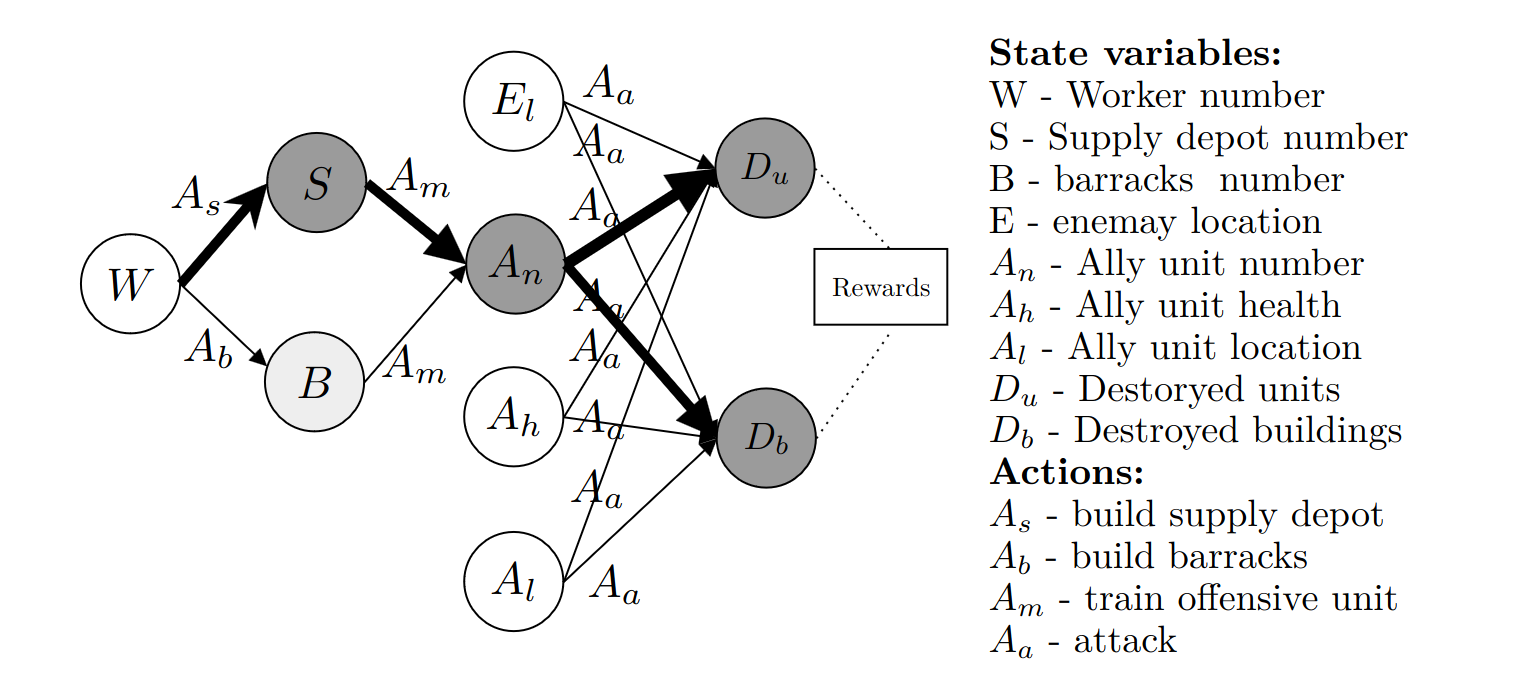
\includegraphics[width=0.9\textwidth]
        {figures/explainability_reinforcement_learning/graph_causal.png}
    \caption{
        Agent--environment interaction model for the video game \textit{StarCraft II} \cite{madumal2020explainable}.
    }
    \label{fig:interaction_model_causal_graph}
\end{figure}


Modeling the interactions between an agent and its environment makes it possible to understand how the agent's decisions are made and what impact they have on the environment (see Figure~\ref{fig:interaction_model_causal_graph}).
By incorporating these interactions into an explanatory model, one can better grasp the complex relationships between the agent and its environment, thereby identifying the determining factors in the decision-making process.
By explicitly handling the agent--environment interaction, this type of explanation aims to explain the agent's strategy.
The methods used to obtain explanations in the form of agent--environment interactions are: \textit{Bayesian network learning} and \textit{latent space usage for MDP generation}.

\subsubsection{\textit{Bayesian Network Learning}}
\label{subsubsec:bayesian_network_learning}

The evolution of an agent within an environment can be observed as a set of \textbf{random variables} connected through a \textbf{Bayesian network} \cite{madumal2020explainable}.
Random variables are defined to represent both external aspects (the environment) and internal aspects of the agent (the actions).
By analyzing trajectories, it becomes possible to infer causal relationships among these random variables.
At the end of this process, a weighted causal graph is obtained, which serves as an explanation for the observer.
This \textit{Bayesian network}, representing the interactions between the agent and the environment, is then used as the explanation.

\subsubsection{\textit{Latent Space Usage for MDP Generation}}
\label{subsubsec:latent_space_mdp_generation}

Each layer of a neural network can be viewed as a projection from one space to another \cite{zahavy2017graying}.
As information propagates through successive layers of a neural network, it becomes increasingly abstract.
It can therefore be assumed that two vectors that are close in this projected space are also close in terms of the agent's perception.
Based on this observation, it is possible to \textbf{redefine an MDP} by leveraging the \textbf{abstract representations} produced by the final layers of a neural network.
Once the new MDP has been constructed, a model of the interaction between the agent and its environment is obtained.
This model, represented as a \textit{graph}, is then used as the explanation.
